\documentclass[12pt,a4paper]{article} 
\usepackage[portuguese]{babel}
\usepackage[utf8]{inputenc}
\usepackage{adjustbox}
\usepackage{graphicx}
\usepackage{booktabs}
\begin{document}
\setcounter{section}{3}
\setcounter{page}{7}
\section{Relatório}
\subsection{Introdução}
Pretende-se neste prática confirmar os comportamentos teorizados a cerca de diodos. Para tal finalidade, mediu-se tensões e resistências diretas e reversas e comparou-se com  os resultados esperados de um dido ideal. Espera-se que $V_t$, a tensão de limiar, do diodo de \emph{Si} seja $0.7 V$ e o diodo de \emph{Ge} seja de $0.3 V$.

Um segundo experimento foi realizado para confirmar a curva característica de um diodo.  Tal experimento foi realizado medindo as diferentes tensões no terminal do diodo, conforme variou-se a tensão de alimentação, $V_{cc}$, de $-12V$ a $+12V$. A figura~\ref{fig:diode_chracteristics} ilustra o comportamento teórico esperado de um diodo, aprensentado a relação entre a corrente e a tensão em seus terminais. Também foram feitas simulações no software \emph{LTspice} para que se possa comparar os resultados obtidos com as curva características dos diodos utilizados em específico. 
\begin{figure}[htpb]
  \centering
  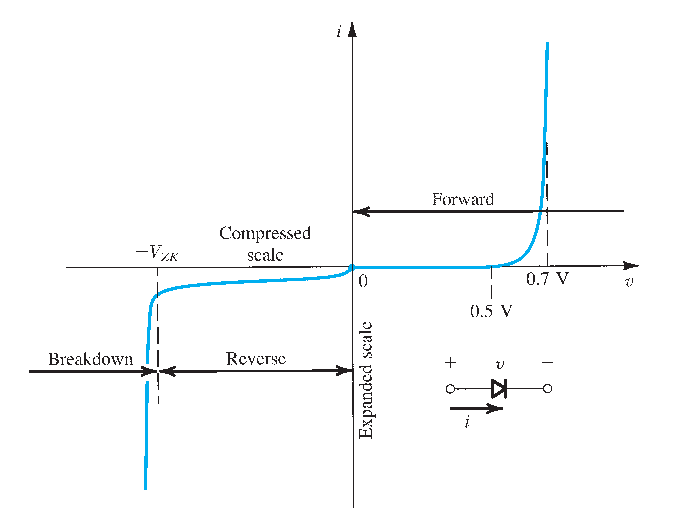
\includegraphics[width=0.8\linewidth]{diode_characteristics.pdf}
  \caption{Curva de funcionamento ideal de um diodo (\emph{Si})}
  \label{fig:diode_chracteristics}
\end{figure}
\subsection{Análises}
Os componentes alvo de nosso estudo foram:
\begin{itemize}
  \item  Diodo 1N4148 (Silício)
  \item  Diodo 1N60 (Germânio)
  \item Diodo Zener 3V3 (Silício)
\end{itemize}
  Como primeiro passo, realizou-se testes com um multímetro digital a fim de estimar os seguintes parâmetros de cada componente; Tensão Direta, Tensão Reversa, Resistência Direta e Resistência Reversa. Tal experimento gerou a Tabela~\ref{tab:1}.
% Os diodos 1N4148 e 1N60 operam na regiâo ativa e o Zener 3V3 trabalha na região zenner. 
% Percebemos na nossa primeira medição que os valores apresentados para tensão direta estão de acordo com nossas expectativas originais, dado que eles se mantiveram em torno de $0.7V$ para diodos compostos de silício e $0.3V$ para o diodo compost de germânio. Também nota-se que o único diodo que apresentou tensão reversa foi o Zenner, que também é um comportamento esperado.

\begin{table}[htpb]
  \centering
  \caption{Teste do diodo}
  \label{tab:1}
  \begin{adjustbox}{max width=\textwidth}
  \begin{tabular}{c c c c c}
    \toprule
    & Tensão Direta ($V$) & Tensão Reversa ($V$) &Resistência Direta ($\Omega$)& Resistência Reversa ($\Omega$)\\ \midrule
    1N4148  &$0.593$ &O.L&26$M$ &O.L  \\
    1N60&0.276 &O.L &198$K$&O.L  \\
    Zener 3V3&0.708 &1.713 &26.5$M$ &21.7$M$\\\bottomrule
  \end{tabular}
\end{adjustbox}
\end{table}
Analisadas as características básicas de cada componente, o circuito relativo a Figura~\ref{fig:1} foi montado na protoboard para os diodos Zener 3V3 e 1N4148. Mediu-se as correntes que passavam nos terminais diodos e a tensão nos terminais do componente, para um tensão de polarização começando em $-12V$ e terminando em  $12 V$, com variações de $1V$. Estas medidas geraram os gráficos da curva característica de cada diodo de forma empírica, representados nas Figura~\ref{fig:2} e Figura~\ref{fig:3} que posteriormente serão comparados com as curvas simuladas.
\begin{figure}[htpb]
  \centering
  \includegraphics{protoboard.pdf}
  \caption{Circuito de análise do diodo utilizado para o \emph{experimento 2}}
  \label{fig:1}
\end{figure}
\begin{figure}[htpb]
  \centering
  \includegraphics[width=0.8\linewidth]{1n4148_characteristics.pdf}
  \caption{Curva característica para o diodo 1N4148 obtida de forma empírica}
  \label{fig:2}
\end{figure}
\begin{figure}[htpb]
  \centering
  \includegraphics[width=0.8\linewidth]{zenner_characteristics.pdf}
  \caption{Curva característica para o diodo Zenner 3v3 obtida de forma empírica}
  \label{fig:3}
\end{figure}
\newpage
\subsection{Discussões}
Observando o comportamento dos nosso gráficos empíricos gerados a partir dos dados no laboratório, Figuras~\ref{fig:2}--\ref{fig:3}, notamos algumas diferenças relativas ao comportamento dos diferentes tipos dos diodos. O diodo Zenner, como esperado, além de operar na região direta, também opera em polarização reversa, assim conduzindo corrente nesta faixa. Observa-se também que a tensão de ruptura pôde ser estimada através de nossos dados como algo perto de $-10V$.

Destes gráficos também observou-se como os diodos se comportam na região ativa, e a partir de quais valores o diodo conduz significamente corrente elétrica, ambos os gráficos nos mostram que este valor foi algo próximo do esperado pela teoria, $0.7V$ para diodos compostos de silício e $0.3V$ para diodos compostos de germânio. 
\begin{figure}[htpb]
  \centering
  \includegraphics[width=0.8\linewidth]{spice_graphic.pdf}
  \caption{Curva característica para o diodo 1N4148 obtida através dos dados do simulador LTspice}
  \label{fig:spice_graphic}
\end{figure}
Ao comparar o gráfico simulado e experimental do diodo 1N4148, Figura~\ref{fig:2} e \ref{fig:spice_graphic}, notamos uma inclinação menos íngrime e uma curva mais suave em na simulação, mas ambos os gráficos apontam as mesmas características essencias como a não há condução na região reversa e que até um valor crítico o diodo se comportou praticamente como um  circuito aberto.

A partir das Figura~\ref{fig:2} e \ref{fig:spice_graphic} podemos modelar nosso diodo como um circuito linear composto de uma fonte de tensão e um resistor, como mostra as Figuras~\ref{fig:circ_equiv} e Figura~\ref{fig:circ_equiv_simul} . O valor escolhido para a resistência foi o inverso da inclinação da reta de cada gráfico dada a partir do eixo $x$ até o ponto $10mA$, nos gerando outras curvas característica equivalente. Tais curvas estâo retratadas nas figuras . Nota-se que na linearização as diferenças entre os resultados simulados e empíricos diminuíram significativamente, confirmando a validade do experimento prático.
\begin{figure}[htpb]
  \centering
  \includegraphics{circ_equiv.pdf}
  \caption{Circuito linear equivalente ao diodo de acordo com os dados experimentais}
  \label{fig:circ_equiv}
\end{figure}
\begin{figure}[htpb]
  \centering
  \includegraphics{circ_equiv_simul.pdf}
  \caption{Circuito linear equivalente ao diodo de acordo com os dados experimentais}
  \label{fig:circ_equiv_simul}
\end{figure}
\begin{figure}[htpb]
  \centering
  \includegraphics[width=0.8\linewidth]{simulado_simplificado.pdf}
  \caption{Curva característica do circuito linear equivalente ao diodo através dos dados de simulação }
  \label{fig:simulado_simplificado}
\end{figure}
\begin{figure}[htpb]
  \centering
  \includegraphics[width=0.8\linewidth]{empirico_simplificado.pdf}
  \caption{Curva característica do circuito linear equivalente ao diodo através dos dados dos dados empíricos}
  \label{fig:empirico_simplificado}
\end{figure}

Ao acessar o datasheet do fabricante, podemos verificar se as tensões encontradas para $10mA$ estão dentro do esperado. A Figura~\ref{fig:datasheet} nos mostra as características a partir do datasheet do Diodo 1N4148, que foram retirados do site da fabricante (Datsheet Reference: \emph{NXP Semiconductors}, 14N4148,  2004 August 10). Nele vemos que $V_f$ deveria estar menor que $1V$, o que acontece para nossos experimentos, já que nossos valores ficaram em torno de $0.7V$.
\begin{figure}[htpb]
  \centering
  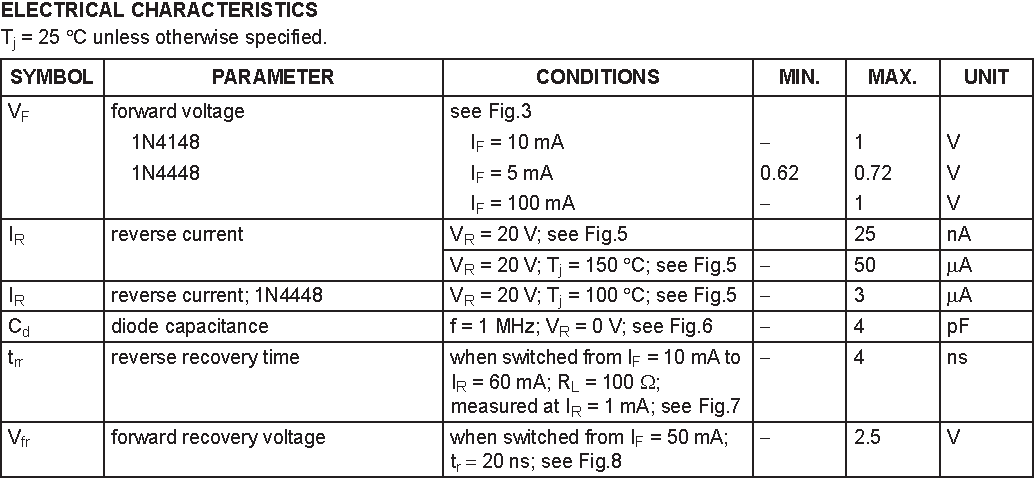
\includegraphics[width=\linewidth]{datasheet.pdf}
  \caption{Parte do datasheet do Diodo 1N4148}
  \label{fig:datasheet}
\end{figure}
\newpage
\subsection{Conclusão}
Nestes experimentos foi possível vislumbrar o funcionamento de diversos tipos de diodo de forma geral, assim como métodos de análise e simplificações que nos possibilita concluir se um diodo está se comportando de maneira esperado pelo seu fabricante. Também certificou-se que o potencial de offset de diodos de germânio é inferior aos de Silício, assim como esperávamos pela teoria.  Aprendeu-se que diodos 1N60 e 1N4148 não operam quando reversamente polarizados, característica que se mostrou ser exclusiva do diodo Zener. Obteu-se também conhecimento de como simular circuitos no software LTspice e como modelar um diodo em uma fonte de tensão e uma pequena resistência. Clarificou-se assim, algumas dúvidas e incertezas que o entendimento da teoria sozinha não havia satisfeito. 
\end{document}
